\section{L'ensemble des entiers naturels}

\subsection{Notation}

Comme leur nom l'indique, les entiers dits "naturels" correspondent aux nombres tels qu'on se les représente de manière naturelle.
Concrètement, ce sont ceux qui nous permettent de compter dans la vie de tous les jours.

D'un point de vue mathématique, on peut définir les entiers naturels comme les nombres strictement positifs qui peuvent s'écrire sans virgule.\\
\\

L'infinité de cet ensemble est intuitive. En effet, en partant de 0, et en comptant de 1 en 1, il apparait évident qu'on pourra toujours rajouter 1, et que le comptage n'aura jamais de fin.

L'infinité de l'ensemble nous oblige donc à avoir recours à une notation spéciale pour le désigner. La notation que nous utilisons encore aujourd'hui nous vient de \textit{Richard Dedekind}\ref{itm:entnat}. Il s'agit d'un N capital, stylisé de la manière suivante : 
$\ens{N}$

\subsection{Quelques propriétés intéressantes}
\subsubsection{Comparaison avec les autres ensembles usuels}

De par sa définition, l'ensemble $\ens{N}$ est le plus évident, mais donc aussi le plus basique des ensembles. Quand les mathématiques se sont complexifiées, d'autres ensembles ont été définis.

L'ensemble des entiers relatifs, noté $\ens{Z}$, comprend l'ensemble $\ens{N}$, auquel s'ajoutent tous les entiers négatifs.

L'ensemble des décimaux, noté $\ens{D}$, comprend tous les nombres pouvant s'écrire sous la forme $\frac{a}{10^b}, \text{avec} \ a \in \ens{Z} \ \text{et} \ b \in \ens{N}$.
Concrètement, on retrouve l'ensemble $\ens{Z}$ pour $b = 0$. 

L'ensemble des rationnels, noté $\ens{Q}$, comprend tous les nombres pouvant s'écrire sous la forme d'une fraction. Autrement dit, il s'agit de tous les nombres qui s'écrivent sous la forme $\frac{a}{b}, \text{avec} \ a \in \ens{Z} \ \text{et} \ b \in \ens{N}$.

L'ensemble des réels, noté $\ens{R}$, comprend l'ensemble des nombres qui peuvent s'écrire avec simplement une partie entière et une liste, potentiellement infinie, de décimales. Cela comprend l'ensemble $\ens{Q}$, ainsi que des nombres tels que $e$ ou $\pi$.\\
\\


Comme nous avons pu le voir, ces ensembles peuvent être vus comme plus ou moins grands, dans la mesure ou certains ensembles sont strictement compris dans d'autres.

En notation mathématique, on peut écrire : 
$\ens{N} \subset \ens{Z} \subset \ens{D} \subset \ens{Q} \subset \ens{R}$

On peut aussi se représenter les choses de façon plus visuelle avec un schéma de ce type (voir figure \ref{fig:schm_ensembles}).

\begin{figure}[h]
    \centering
    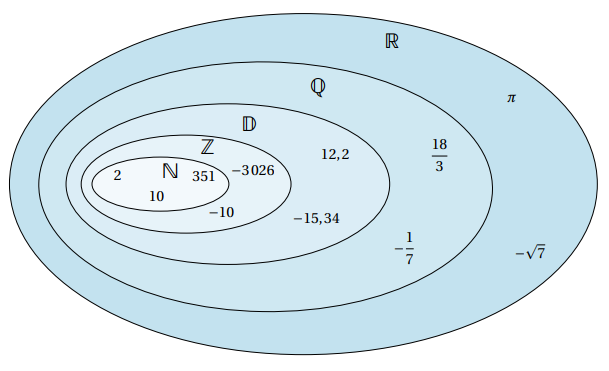
\includegraphics[scale=0.5]{schema_ensembles.png}
    \caption{Schéma Ensembles}
    \label{fig:schm_ensembles}
\end{figure}

(Note : si l'on s'aventure du côté des structures algébrique, on peut remarquer que l'ensemble $\ens{N}$ est le seul ensemble des cinq à ne pas être un groupe\ref{itm:Groupe})

\subsubsection{Infinis dénombrables}

Par son aspect intuitif pour compter, on utilise souvent l'ensemble $\ens{N}$ pour étudier la cardinalité d'un autre ensemble.

\begin{definition}
\textbf{Cardinalité :} \newline
La cardinalité d'un ensemble $E$, notée $card(E)$, correspond au nombre d'élements de $E$.
\end{definition}

\begin{corollary}
\textbf{Ensembles finis} : \newline
$E$ est un ensemble fini si et seulement si $card(E) \in \ens{N}$ .
\end{corollary}

Plus rigoureusement, dire que $card(E)=n$ veut dire que l'on peut faire une bijection\ref{itm:Bijec} entre l'ensemble $E$ et l'ensemble $\{1, \ldots ,n\} \subset \ens{N}$. \newline
\newline
Maintenant que nous avons traité le cas des ensembles finis, regardons quand ces ensembles sont infinis : \newline
\newline
Premièrement, on remarque que l'infini peut contenir l'infini... et peut aussi être contenu dans un autre infini ! ($2\ens{N} \subset \ens{N} \subset \ens{Z}$) \newline
Compliqué de dégager une cardinalité précise de tout ça... \newline
Mais de ce problème s'ensuit une définition fondamentale sur la cardinalité :

\begin{definition}
\textbf{Infinis dénombrables} : \newline
Soit $E$ un enemble infini. S'il existe une bijection entre $E$ et $\ens{N}$, alors on dit que $E$ est un ensemble dénombrable.
On note sa cardinalité par ce signe :
$$Card(\ens{N}) = \aleph_0$$
\end{definition}

Maintenant, avec cette définition, nous avons une réponse pour les cardinalités infinies. \newline
Regardons lesquels des ensembles usuels sont dénombrables :

\begin{theorem}
\label{thm:CrdEnU}
\textbf{Cardinalités des ensembles usuels} : \newline
$$Card(\ens{N})=Card(\ens{Z})=Card(\ens{D})=Card(\ens{Q})$$
\end{theorem}

\begin{proof}
La démonstration étant longue et hors-sujet, elle est donc libre à vous de la trouver par vous même ou d'aller chercher la réponse sur internet !
\end{proof}

Aussi fou que cela puisse paraître, même des ensembles qui paraissent intuitivement bien plus grands possèdent finalement la même cardinalité que $\ens{N}$. \newline
Mais dans le théorème \ref{thm:CrdEnU}, on voit que l'ensemble des Réels manque à l'appel !

\begin{theorem}
\textbf{Infinis indénombrables} : \newline
Il  n'existe aucune bijection entre l'ensemble $\ens{N}$ et l'ensemble $\ens{R}$. \newline
Par conséquent,
\begin{align*}
    Card(\ens{R}) & \not= \aleph_0 \\
    & = c \ \text{("continu")}
\end{align*}

Par définition :
$$2^{\aleph_0} = c$$
\end{theorem}

\begin{proof}
Voir la diagonale de G. Cantor \ref{itm;DiaCan}.
\end{proof}


Et bien finalement si, certains ensembles infinis sont vraiment plus grands que... l'infini. \newline
\newline
Une autre question se pose donc : combien y a-t-il d'infinis ? \newline
Et bien pour l'instant nous n'avons pas encore de réponse. La possible existence d'un cardinal compris entre $\aleph^{0}$ et $\aleph^{1}$ s'appelle \textit{"L'hypothèse du continu"}\ref{itm:HyDuCo}.
\newline
\newline
Conclusion : cet ensemble des plus simples est un puissant outil dans l'analyse des cardinaux.